\section{Part I - Mathematical modeling}\label{sec:part1}

\subsection{Problem 1 - Equations of motion}
\begin{figure}[h]
    \centering
    \begin{subfigure}{0.49\textwidth}
        \centering
        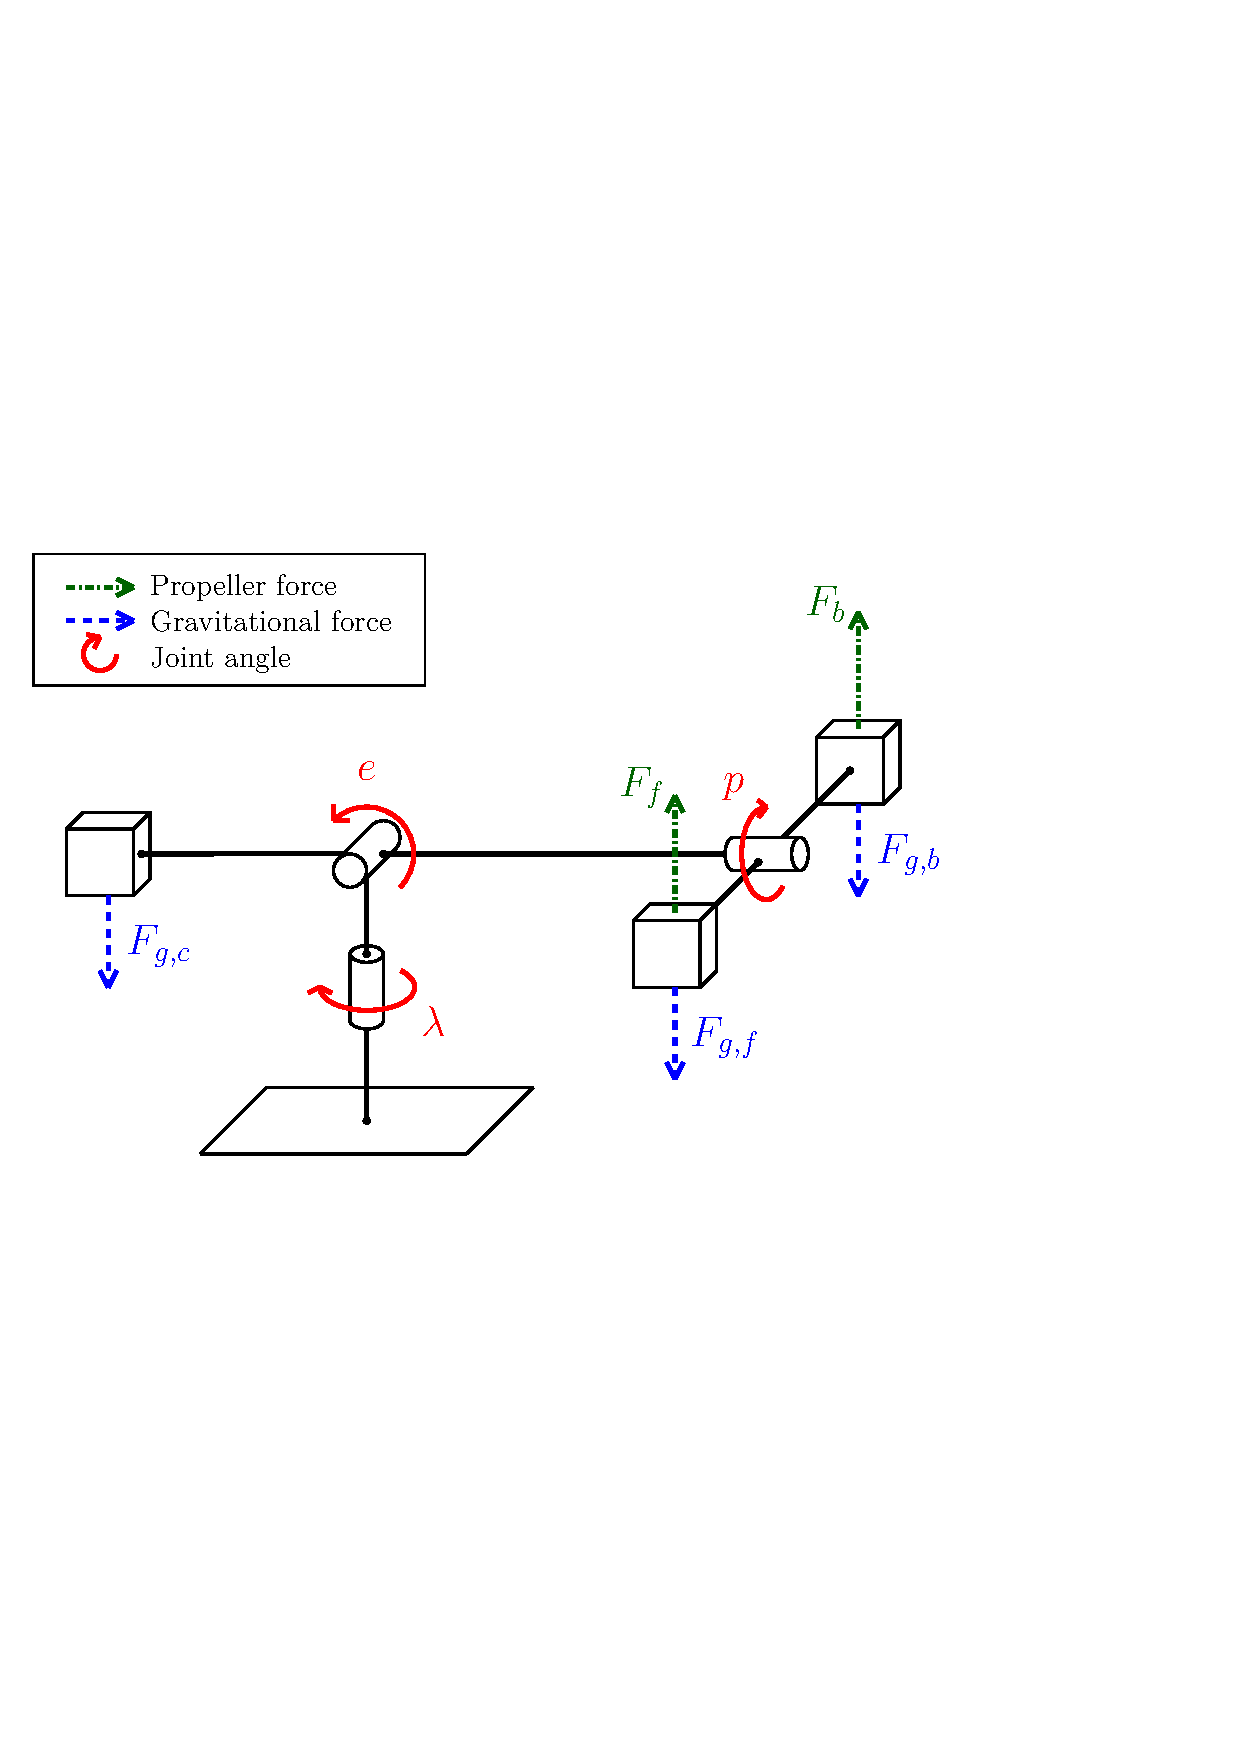
\includegraphics[width = \textwidth]{figures/forces.pdf}
        \caption{Forces on the model}
        \label{fig:forces}
    \end{subfigure}
    \begin{subfigure}{0.49\textwidth}
        \centering
        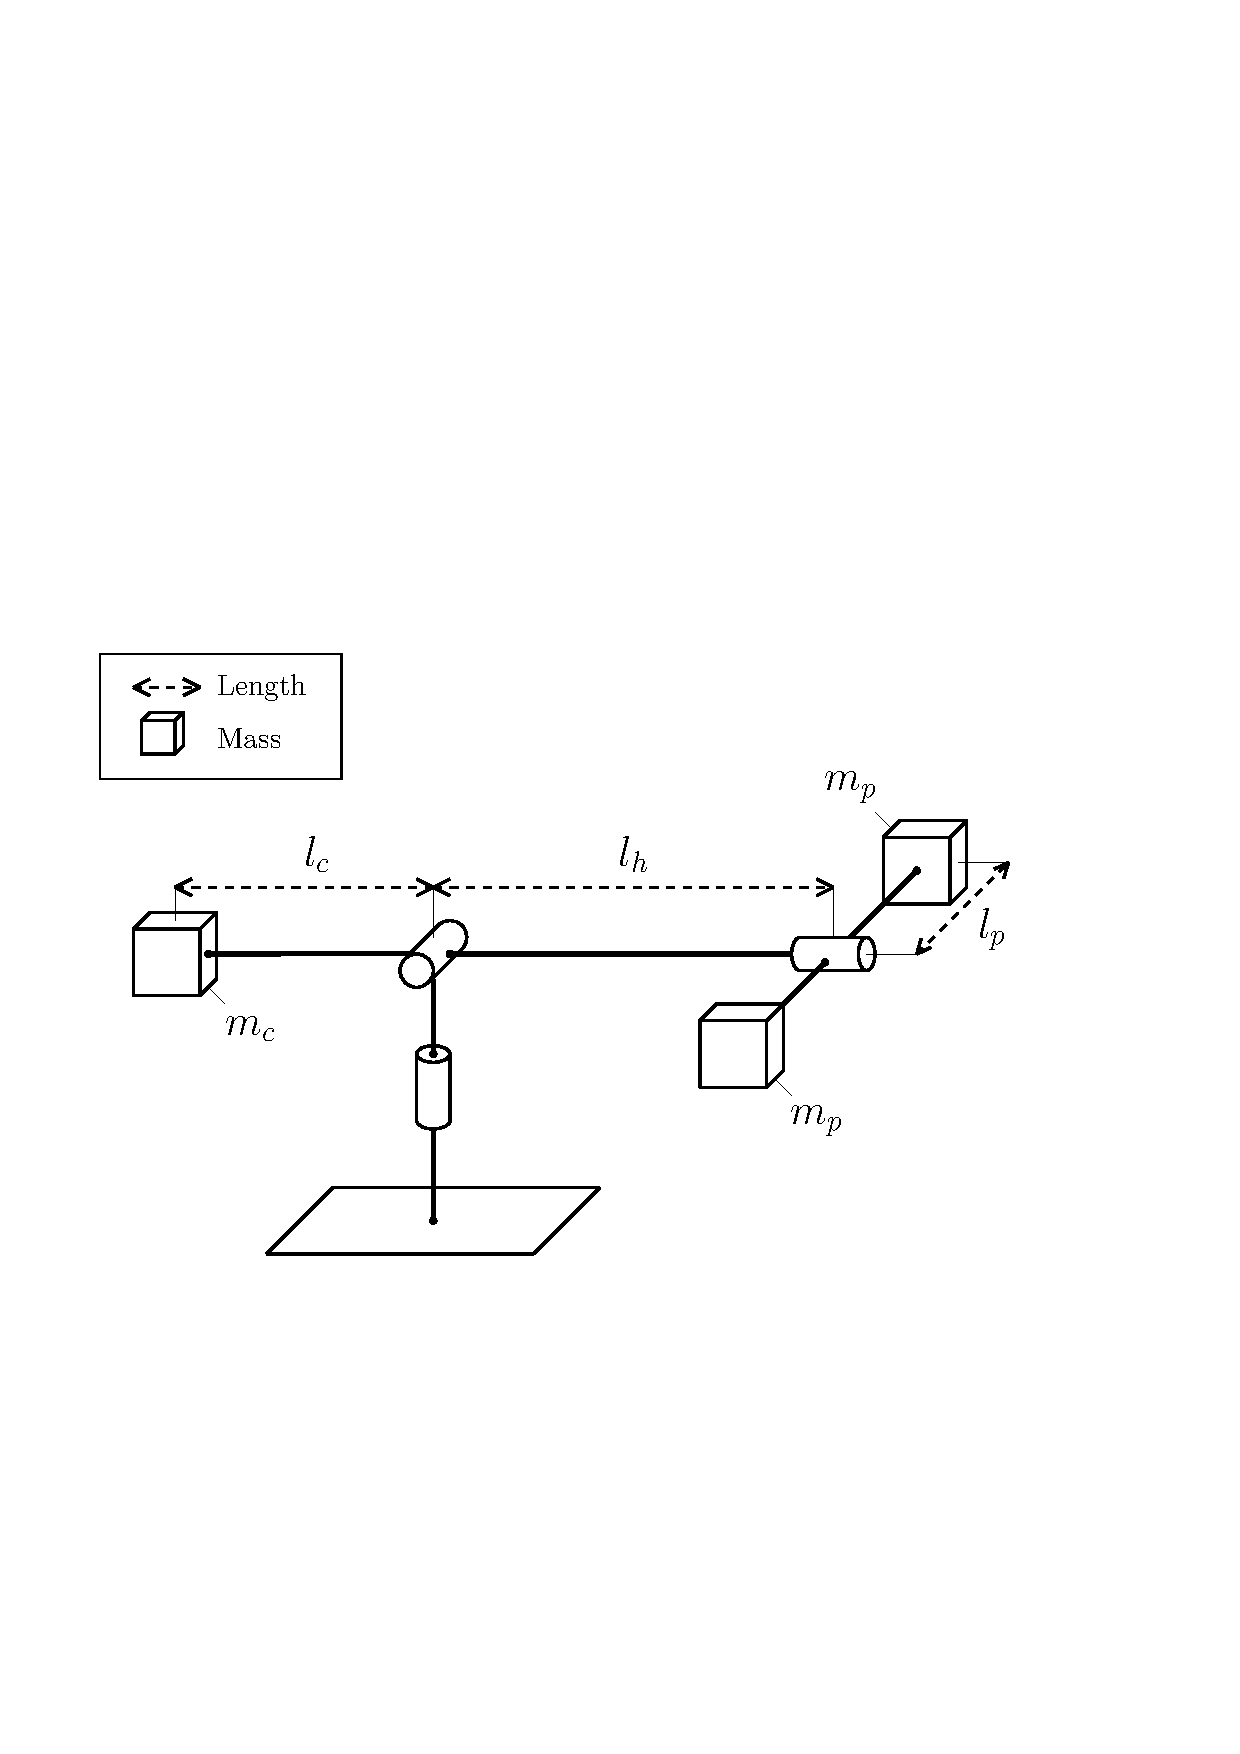
\includegraphics[width = \textwidth]{figures/masses.pdf}
        \caption{Masses and distances}
        \label{fig:masses}
    \end{subfigure}
    \caption{Helicopter model, given in \cite{assignment}}
    \label{fig:model}
\end{figure}
The goal of this problem is to derive the following equations:
\begin{subequations} \label{eq:model}
    \begin{gather}
        J_p \ddot{p} = L_1 V_d \label{eq:model_pitch}\\
        J_e \ddot{e} = L_2 \cos(e) + L_3 V_s \cos(p) \label{eq:model_elev}\\
        J_{\lambda} \ddot{\lambda} = L_4 V_s \cos(e) \sin(p) \label{eq:model_travel}
    \end{gather}
\end{subequations}
These equations lay the foundation of what is the mathematical model of the helicopter.
The force from the motors, front and back, is given by:
\begin{subequations} \label{eq:motor}
    \begin{gather}
        F_f = K_f V_f \label{eq:motor_front} \\
        F_b = K_f V_b \label{eq:motor_back}
    \end{gather}
\end{subequations}
The motor voltages, sum and difference, are defined as:
\begin{subequations}\label{eq:motor_voltage}
    \begin{gather}
        V_s = V_f + V_b \label{motor_voltage_sum}\\
        V_d = V_f - V_b \label{motor_voltage_difference}
    \end{gather}
\end{subequations}
The moments of inertia for pitch, elevation and travel are defined as the following:
\begin{subequations} \label{eq:moments_inertia}
    \begin{align}
        & J_p = 2 m_p l_p^2 \\
        & J_e = m_c l_c^2 + 2 m_p l_h^2 \\
        & J_\lambda = m_c l_c^2 + 2 m_p (l_h^2 + l_p^2)
    \end{align}
\end{subequations}
By using Newton's second low for rotation, we can compute the equations of motion, in the form as stated above. We will insert equation \eqref{eq:motor_front} and \eqref{eq:motor_back}.
\begin{equation} \label{eq:newton2rot}
    J \alpha = \sum{\tau}
\end{equation}
We will begin with the equation for pitch. The torques generated by gravity cancel each other out, so we end up with the torques generated by the motors.
\begin{gather*}
    J_p \ddot{p} = l_p F_{g,b} - l_p F_{g,f} + l_p F_f - l_p F_b \\
    = l_p K_f V_f - l_p K_f V_b = l_p K_f (V_f - V_b) \\
    \implies J_p \ddot{p} = L_1 V_d
\end{gather*}
Now we will look at the equation for elevation. We must use basic trigonometry to find the correct components of the forces. As we can see, the forces are dependant on both pitch angle and elevation angle.
\begin{gather*}
    J_p \ddot{e} = l_c F_{g,c} \cos(e) + l_h (F_f \cos(p) + F_b \cos(p) - l_h F_{g,f} \cos(e) - l_h F_{g,b} \cos(e) \\
    = l_c F_{g,f} \cos(e) + l_h K_f \cos(p) (V_f + V_b) - 2 l_h m_p g \cos(e) \\
    = g(l_c m_c - 2 l_h m_p) \cos(e) + l_h K_f V_s \cos(p) \\
    \implies J_e \ddot{e} = L_2 \cos(e) + L_3 V_s \cos(p)
\end{gather*}
The last equation is the one for travel. Once again, we must use basic trigonometry to find the force and lever arm which are orthogonal. 
\begin{gather*}
    J_\lambda \ddot{\lambda} = \tau_f - \tau_b \\
    = - l_h \cos(e) F_f \sin(p) - l_h \cos(e) F_b \sin(p)\\
    = - l_h K_f (V_f + V_b) \cos(e) \sin(p) = - l_h K_f V_s \cos(e) \sin(p)\\
    \implies J_\lambda \ddot{\lambda} = L_4 V_s \cos(e) \sin(p)
\end{gather*}
So now we also have expressions for the constants $L_{1-4}$:
\begin{subequations}\label{eq:constants-L}
    \begin{align}
        & L_1 = l_p K_f \label{eq:constant-L1}\\
        & L_2 = g (l_c m_c - 2 l_h m_p) \label{eq:constant-L2}\\
        & L_3 = l_h K_f \label{eq:constant-L3} \\
        & L_4 = - L_3 = - l_h K_f \label{eq:constant-L4}
    \end{align}
\end{subequations}
\subsection{Problem 2 - Linearization}\label{subsec:P1p2}
To be able to control our helicopter, we must linearize the equation of motion. We will linearize the model around the point $(p,e,\lambda)^T=(p^*,e^*,\lambda^*)^T$ with $p^*=e^*=\lambda^*=0$. Now we determine the voltages $V_s^*$ and $V_d^*$, such that for all time $\dot{p} = \dot{e} = \dot{\lambda} = 0$. 
This implies that $\ddot{p} = \ddot{e} = \ddot{\lambda} = 0$ for all time. \\
\\Equation \eqref{eq:model_pitch} yields:
\begin{align}
    J_p \cdot 0 = L_1 V_d \implies V_d^* = 0
\end{align}
Equation \eqref{eq:model_elev} yields:
\begin{align}
    J_e \cdot 0 &= L_2 \cos(0) + L_3 V_s^* \cos(0) \nonumber \\
    L_3 V_s^* &= - L_2 \implies V_s^* = -\frac{L_2}{L_3}\label{eq:vs_tilde}
\end{align}
We use the following coordinate transformation to linearize and rewrite the equations of motion. 
\begin{equation}\label{eq: coord_trans}
    \begin{bmatrix} 
        \tilde{p} \\ \tilde{e} \\ \tilde{\lambda}
    \end{bmatrix}
    =
    \begin{bmatrix} 
        p \\ e \\ \lambda
    \end{bmatrix}
    -
    \begin{bmatrix} 
        p^* \\ e^* \\ \lambda^*
    \end{bmatrix}
    \text{ and }
    \begin{bmatrix}
        \tilde{V_s} \\ \tilde{V_d}
    \end{bmatrix}
    =
    \begin{bmatrix}
        V_s \\ V_d
    \end{bmatrix}
    -
    \begin{bmatrix}
        V_s^* \\ V_d^*
    \end{bmatrix}
\end{equation}
This gives us new expressions for the equations of motion.
\begin{subequations}
    \begin{align}
        & \ddot{\tilde{p}} = \frac{L_1}{J_p} \tilde{V_d} \label{eq:trans_model_pitch}\\
        & \ddot{\tilde{e}} = \frac{L_2}{J_e} \cos(\tilde{e}) + \frac{L_3}{J_e}(\tilde{V_s} - \frac{L_2}{L_3}) \cos(\tilde{p})\label{eq:trans_model_elev} \\
        & \ddot{\tilde{\lambda}} = \frac{L_4}{J_\lambda } (\tilde{V_s}-\frac{L_2}{L_3}) \cos(\tilde{e}) \sin(\tilde{p})\label{eq:trans_model_travel}
    \end{align}
\end{subequations}
We set up a state-space model on the following form and linearize the model around $\mathbf{x}_0 = \mathbf{0}$ and $\mathbf{u}_0 = (0, -\frac{L_2}{L_3})^T$.
\begin{equation*}
    \mathbf{\dot{x}} = \mathbf{Ax} + \mathbf{Bu}
\end{equation*}
Where, 
\begin{equation*}
    \mathbf{x} = 
    \begin{bmatrix}
        x_1 \\ x_2 \\ \vdots \\ x_6
    \end{bmatrix}
    =
    \begin{bmatrix}
        \tilde{p} \\ \dot{\tilde{p}} \\ \tilde{e} \\ \dot{\tilde{e}} \\ \tilde{\lambda} \\ \dot{\tilde{\lambda}} \\ 
    \end{bmatrix}
    \text{ and }
    \mathbf{u} =
    \begin{bmatrix}
        \tilde{u_1} \\ \tilde{u_2}
    \end{bmatrix}
    =
    \begin{bmatrix}
        \tilde{V_s} \\ \tilde{V_d}
    \end{bmatrix}
\end{equation*}
Using equation \eqref{eq:trans_model_pitch}, \eqref{eq:trans_model_elev} and \eqref{eq:trans_model_travel} we get the following expression for $\mathbf{\dot{x}}$.
\begin{equation*}
    \mathbf{\dot{x}} = 
    \begin{bmatrix}
        f_1 \\ f_2 \\ \vdots \\ f_6
    \end{bmatrix}
    =
    \begin{bmatrix}
        x_2 \\ \frac{L_1}{J_p}u_2 \\ \frac{L_2}{J_e}\cos(x_3) + \frac{L_3}{J_e} u_1 \cos(x_1) \\ x_6 \\ \frac{L_4}{J_\lambda}u_1 \cos(x_3) \sin(x_1)
    \end{bmatrix}
\end{equation*}
Now we can find the matrices \textbf{A} and \textbf{B}.
\begin{gather*}
    \mathbf{A} = \frac{\partial \mathbf{f}}{\partial \mathbf{x}} = 
    \left.
    \begin{bmatrix}
        \frac{\partial f_1}{\partial x_1} & \cdots &\frac{\partial f_1}{\partial x_6} \\
        \vdots & \ddots & \vdots \\
        \frac{\partial f_6}{\partial x_1} & \cdots & \frac{\partial f_6}{\partial x_6}
    \end{bmatrix}
    \right|_{\mathbf{x_0}, \mathbf{u_0}}
    \text{, }
    \mathbf{B} = \frac{\partial \mathbf{f}}{\partial \mathbf{u}} = 
    \left.
    \begin{bmatrix}
        \frac{\partial f_1}{\partial u_1} & \frac{\partial f_1}{\partial u_2} \\
        \frac{\partial f_6}{\partial u_1} & \frac{\partial f_6}{\partial u_2}
    \end{bmatrix}
    \right|_{\mathbf{x_0}, \mathbf{u_0}}
\end{gather*}
Calculating the partial derivatives and inserting for the points we are linearizing about, we get
\begin{gather}
    \mathbf{A} = 
    \begin{bmatrix}
        0 & 1 & 0 & 0 & 0 & 0 \\
        0 & 0 & 0 & 0 & 0 & 0 \\
        0 & 0 & 0 & 1 & 0 & 0 \\
        0 & 0 & 0 & 0 & 0 & 0 \\
        0 & 0 & 0 & 0 & 0 & 1 \\
        -\frac{L_2 L_4}{J_\lambda L_3} & 0 & 0 & 0 & 0 & 0 \\
    \end{bmatrix}
    \text{ and }
    \mathbf{B} =
    \begin{bmatrix}
        0 & 0 \\
        0 & \frac{L_1}{J_p} \\
        0 & 0 \\
        \frac{L_3}{J_e} & 0\\
        0 & 0 \\
        0 & 0 \\
    \end{bmatrix}
\end{gather}
And this gives us the linearized equations:
\begin{subequations} \label{eq:lin_model}
    \begin{align}
        &\tilde{\ddot{p}} = K_1 \tilde{V_d} \label{eq:lin_model_pitch}\\
        &\tilde{\ddot{e}} = K_2 \tilde{V_s} \label{eq:lin_model_elev}\\
        &\tilde{\ddot{\lambda}} = K_3 \tilde{p} \label{eq:lin_model_travel}
    \end{align}
\end{subequations}
where
\begin{gather}
    K_1 = \frac{L_1}{J_p}, K_2 = \frac{L_3}{J_e} \text{ and } K_3 = -\frac{L_2 L_4}{L_3 J_\lambda}
\end{gather}

\subsection{Problem 3 - Feed forward control}
Attempting to control the helicopter using feed forward proved to be a challenge, just as expected. We added gains to the joystick output in order to make the response easier to handle. We observed that the physical behaviour of the helicopter resembled the mathematical modelling quite well. However, they will never be perfect, as there exists physical parameters that was not included in the model, e.g. drag and friction. This can explain possible discrepancies in the model and real world.

\subsection{Problem 4 - Helicopter at equilibrium}
Now we want to determine the motor voltage constant, $K_f$, by measuring the value of $V_s = V_s^*$ which makes the helicopter maintain the equilibrium value $e = e^* = 0$. We measured the voltage to be $V_s = V_s^* = 6.75 \text{ V}$. 
\\From equation \eqref{eq:vs_tilde}, we have that $V_s^* = -\frac{L_2}{L_3}$. Furthermore, we can expand this expression using equation \eqref{eq:constant-L2} and equation \eqref{eq:constant-L3}, then solve for $K_f$ and finally insert the constant values and the measured value for $V_s^*$. 
\begin{gather}
    V_s^* = -\frac{L_2}{L_3} = \frac{g(2 l_h m_p - l_c m_c)}{l_h K_f}\nonumber\\
    \implies K_f = \frac{g(2 l_h m_p - l_c m_c)}{l_h V_s^*} = 0.148
\end{gather}